\chapter{الكيمياء الفراغية: الكيرالية والمتماكبات}\label{ch:g12:stereochemistry}

لا تتشابه رائحة أوراق النعناع البستاني ورائحة بذور الكراوية في شيء: فالأولى
رائحة العلكة المنعشة، والثانية رائحة خبز الجاودار الدافئة. ومع ذلك \omterm{def:g7:atoms-and-molecules:molecule}{فالجزيء}
المسؤول عن كل من الرائحتين هو الكارفون نفسه، المكوّن من \omterm{def:g7:atoms-and-molecules:atom}{الذرات} نفسها مرتبطةً
بالترتيب نفسه. ولا يختلف الكارفونان إلا كما تختلف يد يسرى عن يد
يمنى: فكل منهما صورة الآخر في المرآة. وأنفنا، المبني من \omterm{def:g7:atoms-and-molecules:molecule}{جزيئات} هي نفسها
«ذات يد»، يميّز بينهما. وفي هذا الفصل نتعلم رؤية \omterm{def:g7:atoms-and-molecules:molecule}{الجزيئات} في ثلاثة أبعاد.

\begin{recall}
شكل \omterm{def:g7:atoms-and-molecules:molecule}{الجزيئات}، والأسافين الممتلئة والمتقطعة التي ترسمها في
الفراغ (\cref{ch:g10:lewis-and-shape}). \omterm{def:g11:organic-skeletons:isomer}{المتماكبات البنيوية}
(\cref{ch:g11:organic-skeletons}). المجموعات الوظيفية
(\cref{ch:g11:functional-groups}).
\end{recall}

\begin{omfigure}
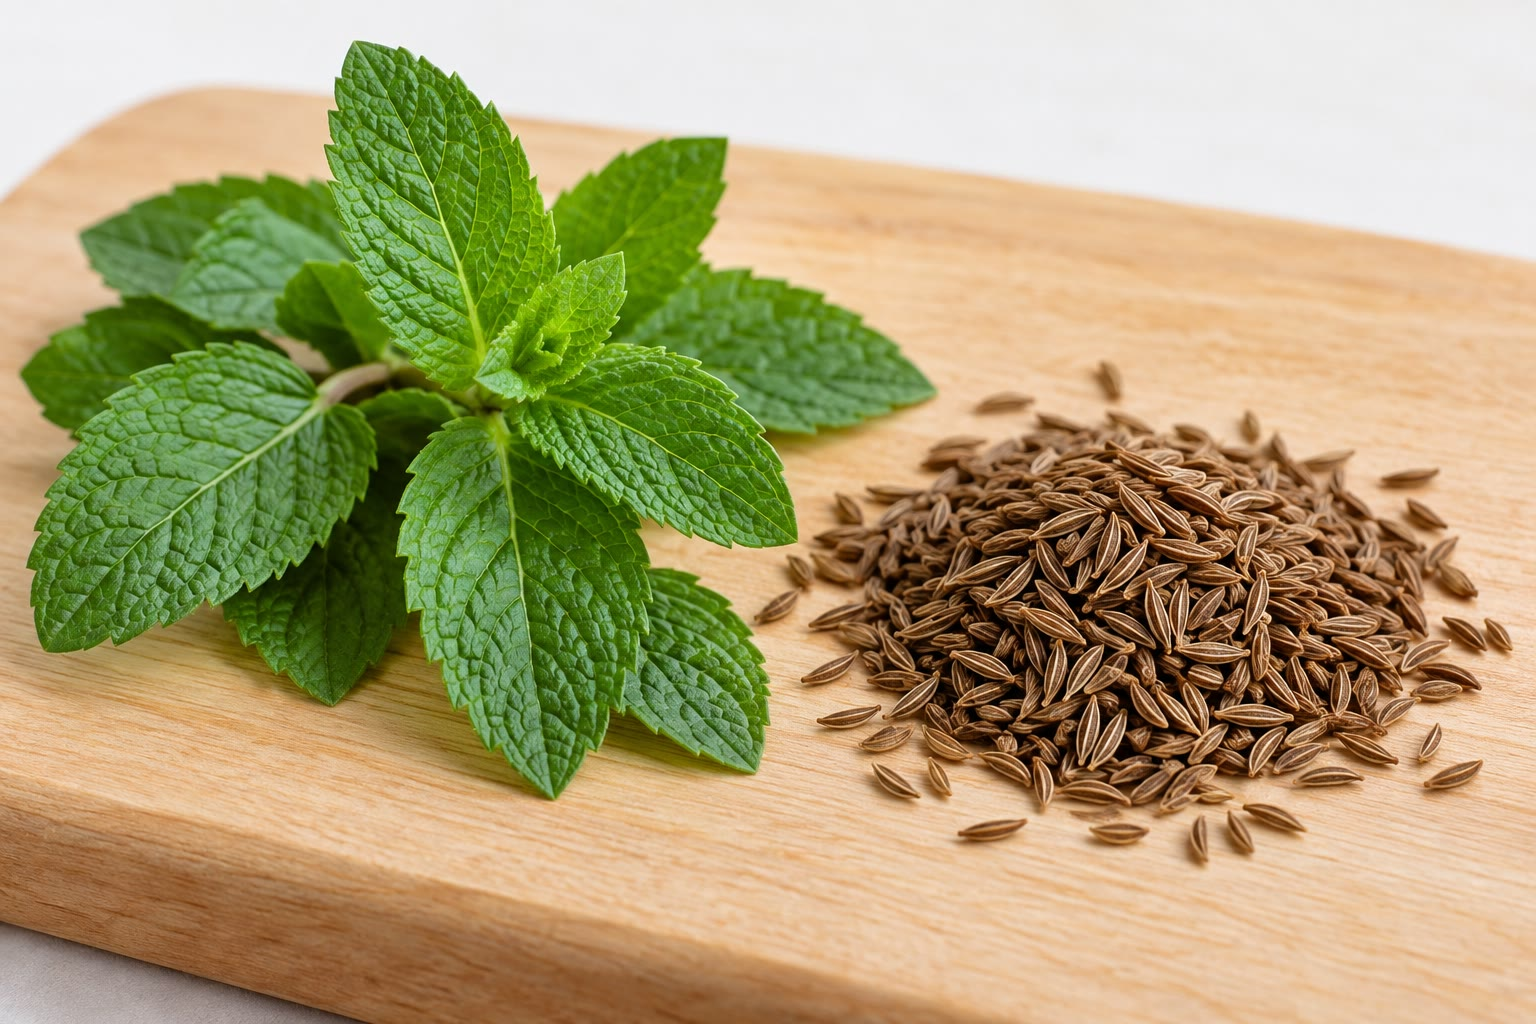
\includegraphics[width=0.48\linewidth]{images/book1/ai/g12-mint-caraway.jpg}

{\small النعناع البستاني والكراوية: جزيئان كلٌّ منهما صورة الآخر في المرآة، ورائحتان.}
\end{omfigure}

\section{الجزيئات في الفراغ}

\begin{definition}[المتماكبات الفراغية]\label{def:g12:stereochemistry:stereoisomer}
\emph{المتماكبات الفراغية}\index{متماكبات فراغية} \omterm{def:g7:atoms-and-molecules:molecule}{جزيئات} لها الصيغة نفسها
وتسلسل \omterm{def:g7:atoms-and-molecules:atom}{الذرات} المترابطة نفسه، ولا تختلف إلا في
ترتيب ذراتها في الفراغ.
\end{definition}

\begin{definition}[تمثيل كرام]\label{def:g12:stereochemistry:cram}
في \emph{تمثيل كرام}\index{تمثيل كرام} \omterm{def:g7:atoms-and-molecules:atom}{لذرة} كربون
ذات أربع روابط أحادية، تُرسم رابطتان في مستوى
الورقة خطين عاديين بينهما زاوية، والرابطة المتجهة نحو القارئ
إسفينًا ممتلئًا والرابطة المتجهة بعيدًا عنه إسفينًا متقطعًا.
\end{definition}

\section{الكيرالية}

\begin{definition}[الكيرالي، الكربون غير المتناظر]\label{def:g12:stereochemistry:chiral}
يكون الجسم أو \omterm{def:g7:atoms-and-molecules:molecule}{الجزيء} \emph{كيراليًا}\index{كيرالي} إذا تعذّر
تطبيقه على صورته في المرآة، كاليد. \omterm{def:g7:atoms-and-molecules:atom}{وذرة} الكربون المرتبطة بأربع
\omterm{def:g7:atoms-and-molecules:atom}{ذرات} أو مجموعات مختلفة \emph{كربون غير
متناظر}\index{كربون غير متناظر}؛ وكثيرًا ما تُميَّز بنجمة.
\end{definition}

\begin{proposition}[كربون واحد غير متناظر يجعل الجزيء كيراليًا]\label{prop:g12:stereochemistry:one-carbon}
\omterm{def:g7:atoms-and-molecules:molecule}{الجزيء} الذي فيه \omterm{def:g7:atoms-and-molecules:atom}{ذرة} كربون غير متناظرة واحدة بالضبط \omterm{def:g7:atoms-and-molecules:molecule}{جزيء} \omterm{def:g12:stereochemistry:chiral}{كيرالي}.
\end{proposition}

\begin{proof}
نقبله: فتبديل اثنتين من المجموعات الأربع المختلفة حول
\omterm{def:g12:stereochemistry:chiral}{الكربون غير المتناظر} يعطي الصورة المرآوية، ولا يمكن لأي دوران \omterm{def:g7:atoms-and-molecules:molecule}{للجزيء}
كله أن يعيدها إلى الأصل، لأن المجموعات الأربع كلها مختلفة.
\end{proof}

\begin{definition}[المتماكبان المرآويان، الخليط الراسيمي]\label{def:g12:stereochemistry:enantiomer}
المتماكبان الفراغيان اللذان كلٌّ منهما صورة الآخر في المرآة ولا
ينطبقان هما \emph{متماكبان مرآويان}\index{متماكبات مرآوية}. \omterm{def:g6:pure-substances-and-mixtures:mixture}{والخليط} من
كميتين متساويتين من متماكبين مرآويين \emph{خليط
راسيمي}\index{خليط راسيمي}.
\end{definition}

\begin{omfigure}
\setchemfig{atom sep=2.2em}
\begin{tikzpicture}[font=\small]
  \node at (-2.4,0) {\chemfig{C(-[2]COOH)(-[4]H_3C)(<[:-30]OH)(<:[:-150]H)}};
  \node at (2.4,0) {\chemfig{C(-[2]COOH)(-[0]CH_3)(<[:-150]HO)(<:[:-30]H)}};
  \draw[dashed, omDef, thick] (0,-1.5) -- (0,1.6) node[above] {مرآة};
  \node[anchor=north] at (-2.4,-1.4) {\foreignlanguage{arabic}{حمض اللبنيك، \babelsublr{A}}};
  \node[anchor=north] at (2.4,-1.4) {\foreignlanguage{arabic}{صورته المرآوية، \babelsublr{B}}};
\end{tikzpicture}

{\small \omterm{def:g12:stereochemistry:enantiomer}{المتماكبان المرآويان} لحمض اللبنيك، \ce{CH3-CH(OH)-COOH}، \omterm{def:g12:stereochemistry:cram}{بتمثيل
كرام}. الكربون المركزي غير متناظر (\ce{H}، \ce{OH}،
\ce{CH3}، \ce{COOH}). ولا يحوّل أي دوران A إلى B: فهما مختلفان
اختلاف اليد اليسرى عن اليمنى.}
\end{omfigure}

\begin{method}[هل الجزيء كيرالي؟]\label{met:g12:stereochemistry:chiral}
\begin{enumerate}
  \item ابحث عن \omterm{def:g7:atoms-and-molecules:atom}{ذرات} الكربون غير المتناظرة: كربون يحمل أربع مجموعات
        مختلفة. فإن لم توجد: \omterm{def:g7:atoms-and-molecules:molecule}{فالجزيء} (في هذا الكتاب) غير \omterm{def:g12:stereochemistry:chiral}{كيرالي}.
  \item واحدة بالضبط: \omterm{def:g7:atoms-and-molecules:molecule}{فالجزيء} \omterm{def:g12:stereochemistry:chiral}{كيرالي}.
  \item اثنتان أو أكثر: ابحث عن مستوى يقسم \omterm{def:g7:atoms-and-molecules:molecule}{الجزيء} إلى نصفين
        كلٌّ منهما صورة الآخر في المرآة، في أحد أشكاله؛ فإن وُجد كان
        \omterm{def:g7:atoms-and-molecules:molecule}{الجزيء} غير \omterm{def:g12:stereochemistry:chiral}{كيرالي}، وإلا فهو \omterm{def:g12:stereochemistry:chiral}{كيرالي}.
\end{enumerate}
\end{method}

\begin{remark}[الخواص نفسها، والروائح مختلفة]\label{rem:g12:stereochemistry:same}
% ledger: smell:carvone-R, smell:carvone-S
للمتماكبين المرآويين درجتا الانصهار والغليان نفسهما، \omterm{def:g6:solutions-and-solubility:solubility}{والذوبانية}
نفسها، والأطياف نفسها: فكل قياس يُجرى بشيء
غير \omterm{def:g12:stereochemistry:chiral}{كيرالي} يعطي النتيجة نفسها لكليهما. ولا يختلفان إلا
حين يلتقيان بشيء \omterm{def:g12:stereochemistry:chiral}{كيرالي}، كالضوء المستقطب، الذي
يديرانه في اتجاهين متعاكسين، أو مستقبلات الأنف: فأحد الكارفونين
رائحته رائحة النعناع البستاني، ومتماكبه المرآوي رائحته رائحة الكراوية.
\end{remark}

\section{المتماكبات اللامرآوية}

\begin{definition}[المتماكبات اللامرآوية]\label{def:g12:stereochemistry:diastereomer}
\omterm{def:g12:stereochemistry:stereoisomer}{المتماكبات الفراغية} التي ليس أحدها صورة الآخر في المرآة هي
\emph{متماكبات لامرآوية}\index{متماكبات لامرآوية}. وخلافًا \omterm{def:g12:stereochemistry:enantiomer}{للمتماكبات المرآوية}،
\omterm{def:g11:organic-skeletons:isomer}{للمتماكبات} اللامرآوية خواص فيزيائية مختلفة.
\end{definition}

\begin{proposition}[عدّ المتماكبات الفراغية]\label{prop:g12:stereochemistry:count}
\omterm{def:g7:atoms-and-molecules:molecule}{للجزيء} الذي فيه $n$ \omterm{def:g7:atoms-and-molecules:atom}{ذرة} كربون غير متناظرة $2^n$ متماكبًا فراغيًا على الأكثر.
ويكون عددها أقل حين يكون \omterm{def:g7:atoms-and-molecules:molecule}{للجزيء} نصفان متماثلان: فيكون لإحدى
التركيبات مستوى مرآة ولا تكون كيرالية (شكل \emph{ميزو}).
\end{proposition}

\begin{proof}
لكل \omterm{def:g12:stereochemistry:chiral}{كربون غير متناظر} ترتيبان ممكنان، باستقلال عن
غيره: $2 \times 2 \times \dots \times 2 = 2^n$ تركيبة. وحين تكون
تركيبتان الجزيءَ نفسه، ينقص العدد.
\end{proof}

\begin{omfigure}
\setchemfig{atom sep=1.9em}
\begin{tabular}{ccc}
\chemfig{HOOC-[:-30]C(<[:-90]OH)-[:30]C(<[:90]OH)-[:-30]COOH} &
\chemfig{HOOC-[:-30]C(<:[:-90]OH)-[:30]C(<:[:90]OH)-[:-30]COOH} &
\chemfig{HOOC-[:-30]C(<[:-90]OH)-[:30]C(<:[:90]OH)-[:-30]COOH} \\[4pt]
\small حمض الطرطريك L & \small حمض الطرطريك D & \small حمض الطرطريك ميزو \\
\small (\omterm{def:g12:stereochemistry:chiral}{كيرالي}) & \small (\omterm{def:g12:stereochemistry:chiral}{كيرالي}، صورة L في المرآة) & \small (غير \omterm{def:g12:stereochemistry:chiral}{كيرالي})
\end{tabular}

{\small \omterm{def:g12:stereochemistry:stereoisomer}{المتماكبات الفراغية} الثلاثة لحمض الطرطريك. L وD \omterm{def:g12:stereochemistry:enantiomer}{متماكبان
مرآويان}؛ وكل منهما متماكب لامرآوي لشكل الميزو، الذي له
مستوى مرآة في أحد أشكاله: ثلاثة \omterm{def:g12:stereochemistry:stereoisomer}{متماكبات فراغية}، لا $2^2 = 4$.}
\end{omfigure}

\begin{history}[باستور يفرز البلورات بيده، 1848]
في سنة 1848 نظر الكيميائي الشاب لويس باستور بعدسة مكبّرة إلى
بلورات ملح من «حمض الراسيميك»، وهو شكل من حمض الطرطريك لا
يدير الضوء المستقطب في أي اتجاه. فلاحظ أن البلورات تأتي على
شكلين، كلٌّ منهما صورة الآخر في المرآة، ففرزها واحدةً واحدةً بملقط.
فلما أذابها، أدارت إحدى الكومتين الضوء المستقطب إلى اليمين، وأدارته
الأخرى، بالمقدار نفسه، إلى اليسار: فحمض الراسيميك \omterm{def:g6:pure-substances-and-mixtures:mixture}{خليط} من جزيئين كلٌّ منهما
صورة الآخر في المرآة. فاستنتج أن \omterm{def:g7:atoms-and-molecules:molecule}{الجزيئات} يمكن أن تكون «ذات يد».
\end{history}

\begin{omfigure}
\begin{minipage}[t]{0.36\linewidth}\centering
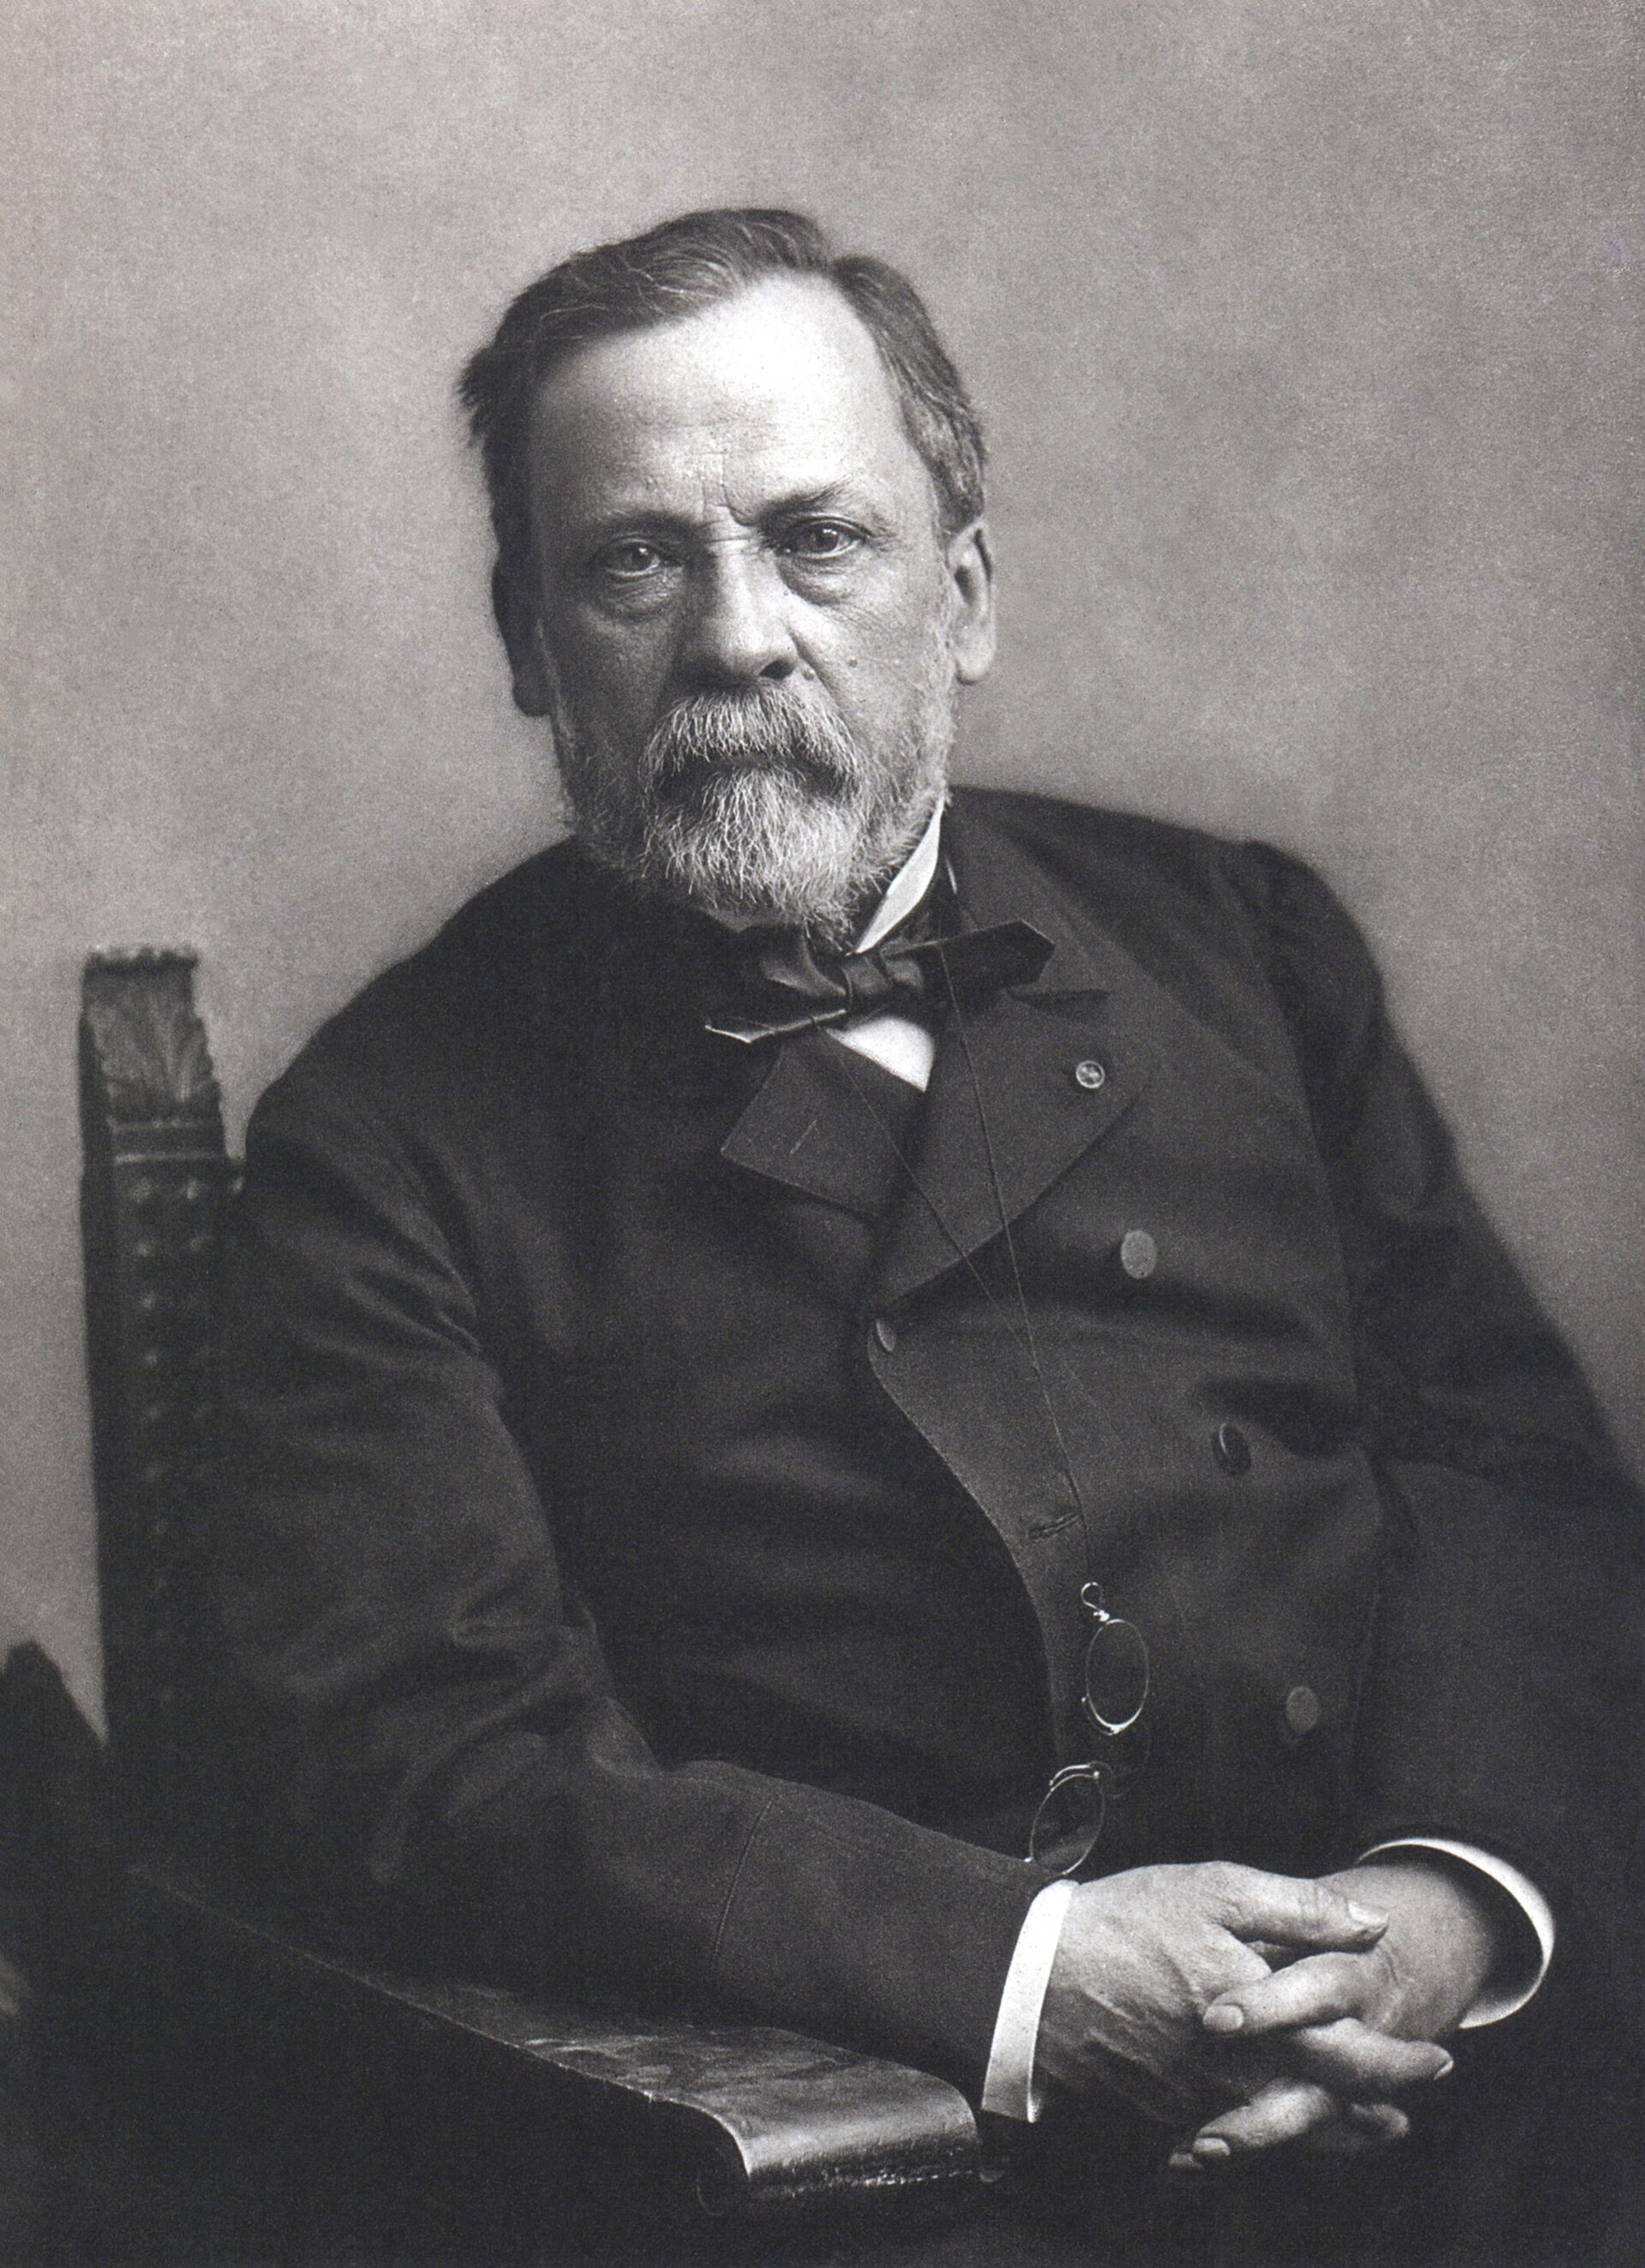
\includegraphics[height=5cm]{images/book1/pasteur.jpg}

{\small لويس باستور (1822--1895)، صوّره بول نادار.}
\end{minipage}\qquad
\begin{minipage}[t]{0.36\linewidth}\centering
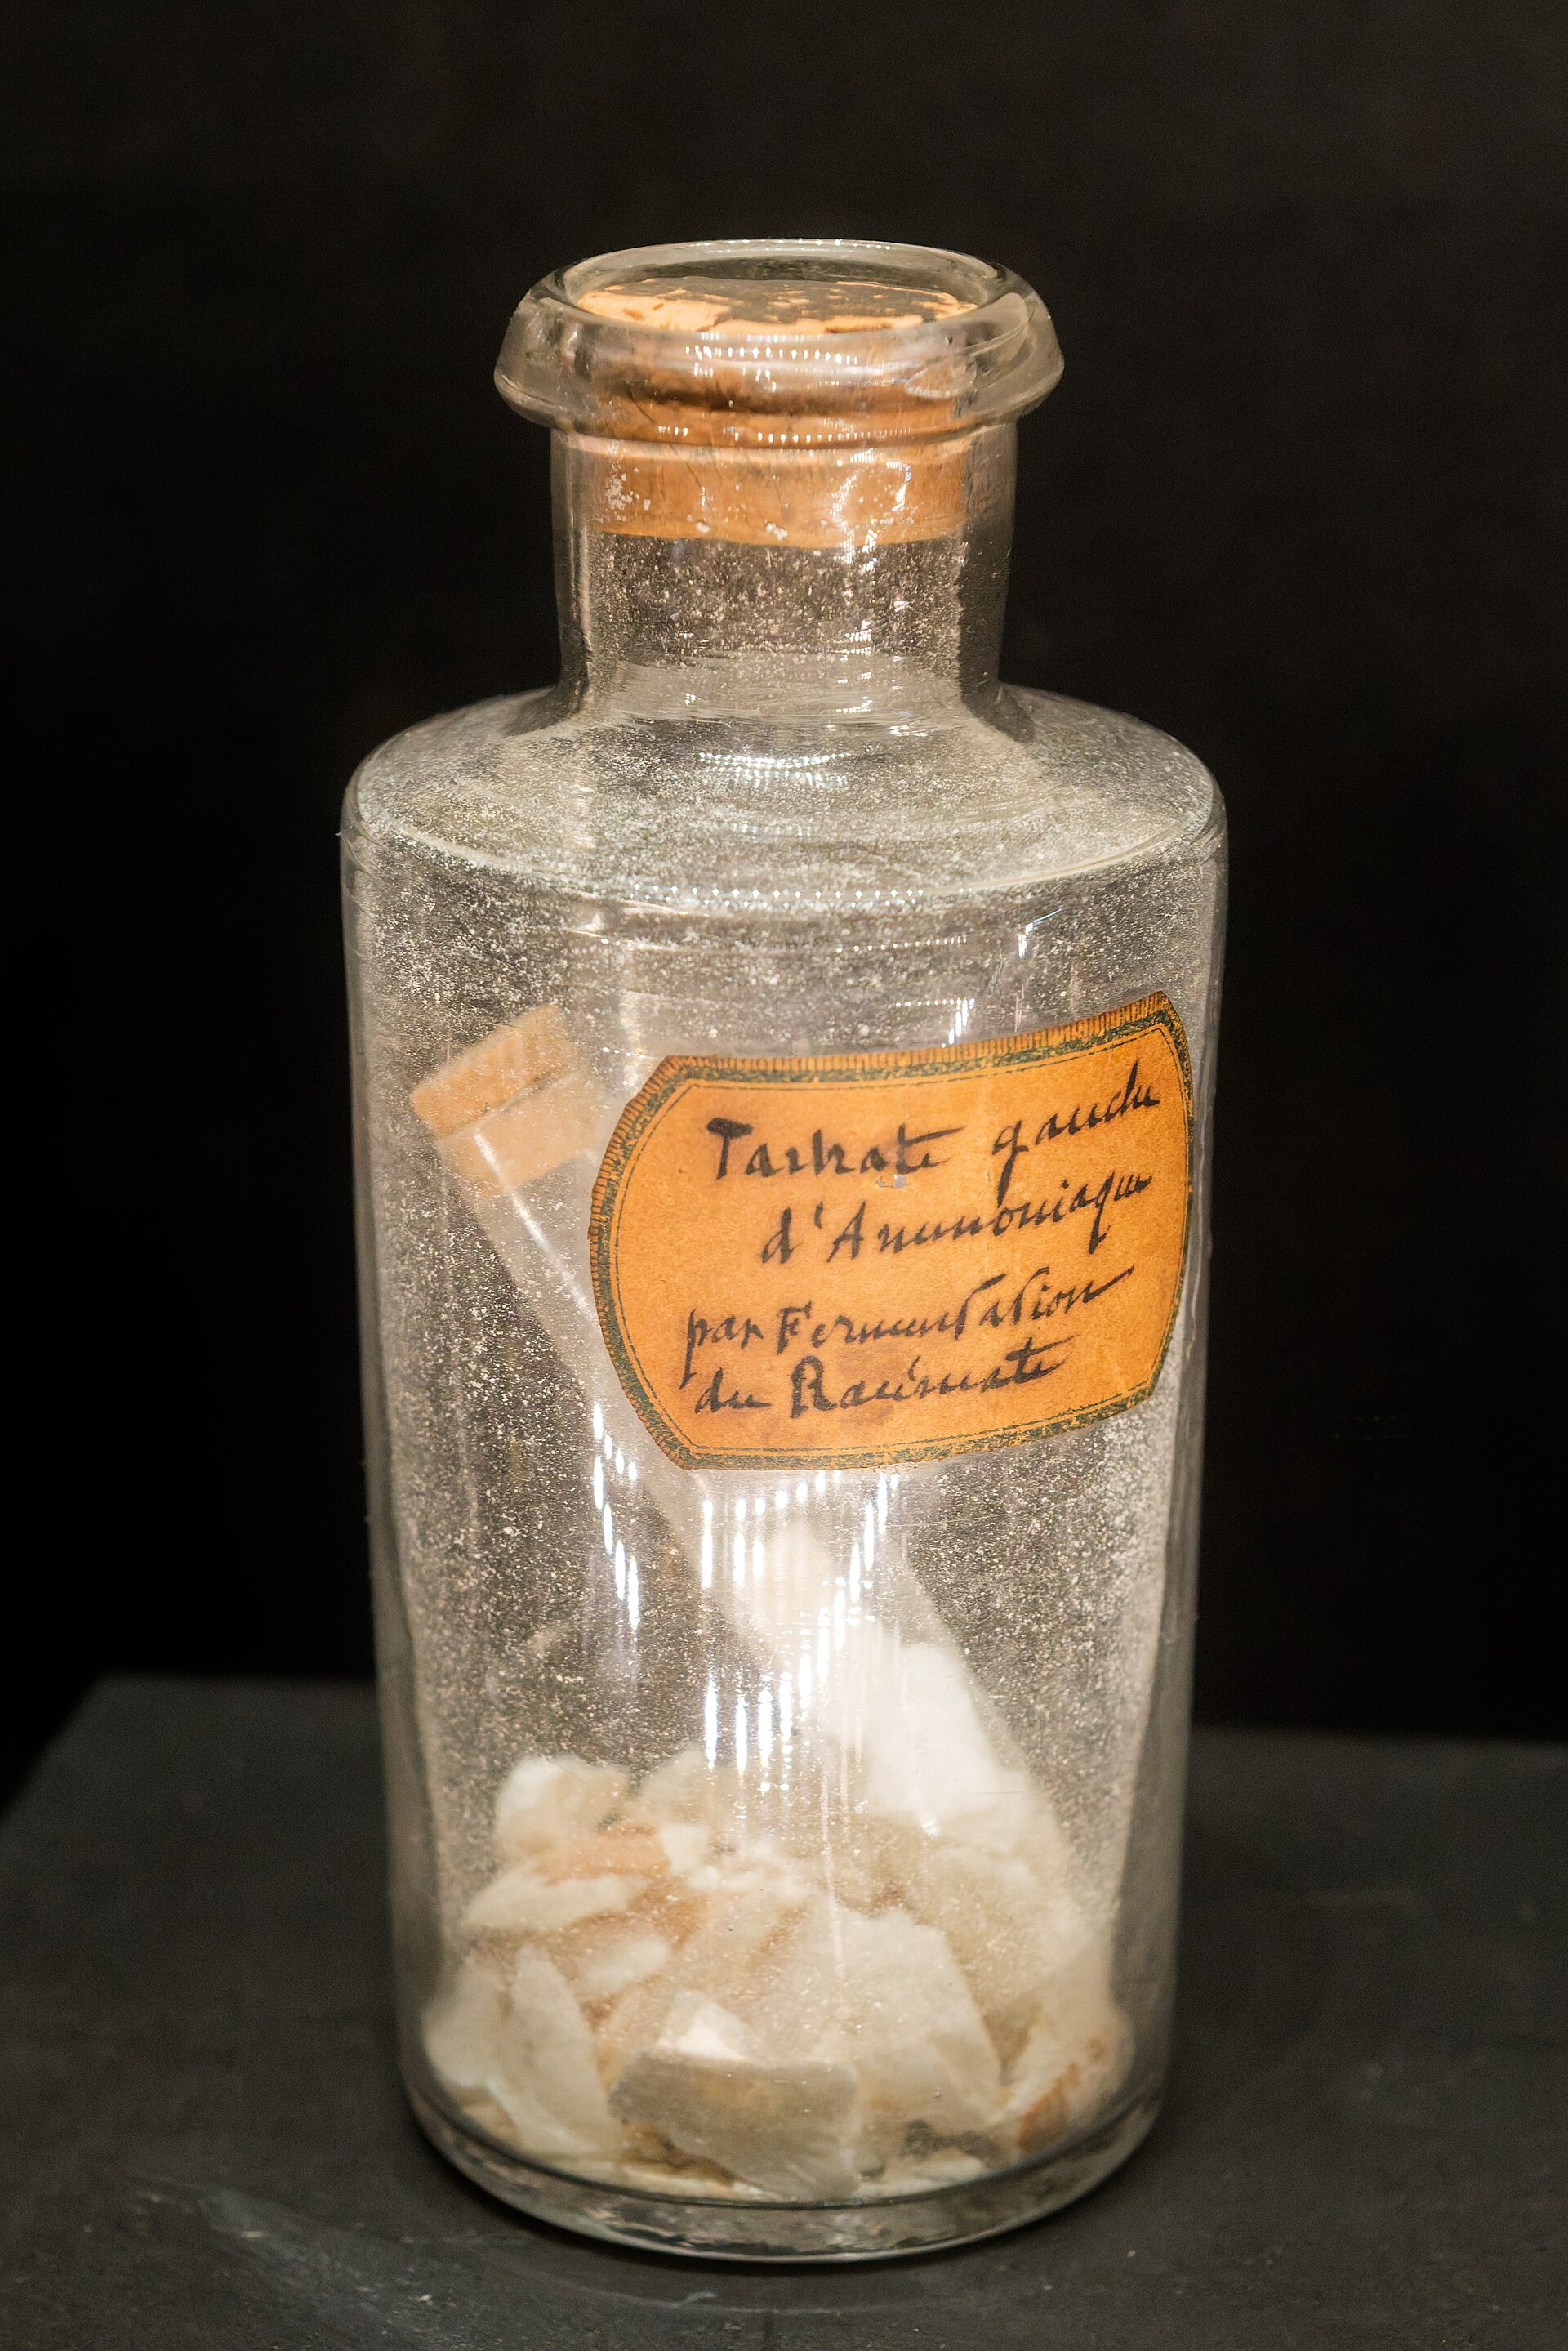
\includegraphics[height=5cm]{images/book1/tartrate-crystals.jpg}

{\small بلورات طرطرات الأمونيوم من مجموعة باستور. تصوير
ماري-لان تاي بامار، CC BY 4.0.}
\end{minipage}
\end{omfigure}

\section{المتماكبان Z وE}


\begin{definition}[المتماكبان Z وE]\label{def:g12:stereochemistry:z-e}
حين تحمل كل \omterm{def:g7:atoms-and-molecules:atom}{ذرة} كربون في \omterm{def:g10:lewis-and-shape:multiple-bond}{رابطة ثنائية} \ce{C=C} ذرتين أو مجموعتين
مختلفتين، يوجد متماكبان فراغيان، لأن \omterm{def:g10:lewis-and-shape:multiple-bond}{الرابطة الثنائية} لا
تدور. وعلى كل كربون تكون الأولوية للمجموعة التي لذرتها المرتبطة به \omterm{def:g9:inside-the-atom:atomic-number}{العدد
الذري} الأكبر. فإذا كانت مجموعتا الأولوية في الجهة نفسها
من \omterm{def:g10:lewis-and-shape:multiple-bond}{الرابطة الثنائية}، كان المتماكب \emph{Z}\index{متماكب Z}؛ وإذا كانتا
في جهتين متقابلتين، كان \emph{E}\index{متماكب E}.
\end{definition}

\begin{method}[Z أم E؟]\label{met:g12:stereochemistry:z-e}
\begin{enumerate}
  \item تحقق من أن كل كربون في \omterm{def:g10:lewis-and-shape:multiple-bond}{الرابطة الثنائية} يحمل مجموعتين
        مختلفتين؛ وإلا فلا تماكب Z/E.
  \item على كل كربون، أعطِ الأولوية للمجموعة التي لذرتها الأولى
        \omterm{def:g9:inside-the-atom:atomic-number}{العدد الذري} الأكبر (والقواعد الكاملة لحالات التساوي في
        مجلد السنة الأولى).
  \item الجهة نفسها: Z. جهتان متقابلتان: E.
\end{enumerate}
\end{method}

\begin{omfigure}
\setchemfig{atom sep=2em}
\begin{tabular}{cc}
\chemfig{C(-[:150]H_3C)(-[:210]H)=C(-[:30]CH_3)(-[:-30]H)} &
\chemfig{C(-[:150]H_3C)(-[:210]H)=C(-[:30]H)(-[:-30]CH_3)} \\[4pt]
\small (Z)-بوت-2-ين: مجموعتا \ce{CH3} في الجهة نفسها &
\small (E)-بوت-2-ين: مجموعتا \ce{CH3} في جهتين متقابلتين
\end{tabular}

{\small المتماكبان الفراغيان للبوت-2-ين. على كل كربون، للمجموعة \ce{CH3}
(كربون، $Z = 6$) الأولوية على \ce{H} ($Z = 1$). وهما
متماكبان لامرآويان: يغليان عند درجتين مختلفتين.}
\end{omfigure}

\section{التشكّلات}

\begin{definition}[التشكّل]\label{def:g12:stereochemistry:conformation}
يمكن \omterm{def:g7:atoms-and-molecules:atom}{لذرات} \omterm{def:g7:atoms-and-molecules:molecule}{الجزيء} أن تدور حول رابطة أحادية. وكل ترتيب
يُبلغ بهذه الدورانات \emph{تشكّل}\index{تشكّل} من تشكّلات
\omterm{def:g7:atoms-and-molecules:molecule}{الجزيء}. وتشكّلات \omterm{def:g7:atoms-and-molecules:molecule}{الجزيء} الواحد ليست \omterm{def:g11:organic-skeletons:isomer}{متماكبات}: فهي يتحول بعضها
إلى بعض باستمرار عند درجة حرارة الغرفة.
\end{definition}

\begin{omfigure}
\begin{tikzpicture}[font=\small]
  \pic (s) at (0,0) {omnewman={90}{30}};
  \foreach \k in {1,2,3} { \node at (s-f\k) {H}; \node at (s-b\k) {H}; }
  \node[anchor=north, align=center] at (0,-1.7) {\foreignlanguage{arabic}{متعاقب: ذرات \babelsublr{H}}\\ للكربونين تتناوب};
  \pic (e) at (5,0) {omnewman={90}{112}};
  \foreach \k in {1,2,3} { \node at (e-f\k) {H}; \node[black!60] at (e-b\k) {H}; }
  \node[anchor=north, align=center] at (5,-1.7) {مكسوف: تتقابل\\ (مرسومة متباعدة قليلًا)};
\end{tikzpicture}

{\small تشكّلان للإيثان، \ce{CH3-CH3}، منظورًا إليهما على امتداد الرابطة
\ce{C-C}: الكربون الأمامي هو المركز، والكربون الخلفي هو الدائرة.
\omterm{def:g12:stereochemistry:conformation}{والتشكّل} المتعاقب، حيث تكون \omterm{def:g7:atoms-and-molecules:atom}{الذرات} أبعد ما يمكن بعضها عن بعض، هو
الأكثر استقرارًا.}
\end{omfigure}

\begin{remark}[لماذا يهم ذلك]\label{rem:g12:stereochemistry:matters}
الكائنات الحية مبنية من \omterm{def:g7:atoms-and-molecules:molecule}{جزيئات} كيرالية (البروتينات، السكريات)،
والمستقبلات والإنزيمات المصنوعة منها تميّز \omterm{def:g12:stereochemistry:enantiomer}{المتماكبات المرآوية}: فقد يختلف
\omterm{def:g12:stereochemistry:enantiomer}{متماكبان مرآويان} اختلافًا كبيرًا في الرائحة أو الطعم أو الأثر الدوائي. ولذلك
على الكيميائيين الذين يصنعون دواءً فيه \omterm{def:g12:stereochemistry:chiral}{كربون غير متناظر} أن يعرفوا
أي متماكب مرآوي يصنعون، وأن يختبروا كلًّا منهما.
\end{remark}

\section{تمارين}

\begin{exercise}[$\star$]\label{exo:g12:stereochemistry:1}
أي هذه \omterm{def:g7:atoms-and-molecules:molecule}{الجزيئات} فيه \omterm{def:g12:stereochemistry:chiral}{كربون غير متناظر}؟ ميّزه بنجمة.
بوتان-2-ول \ce{CH3-CH(OH)-CH2-CH3}؛ بروبان-2-ول \ce{CH3-CH(OH)-CH3}؛
2-كلورو بوتان؛ حمض اللبنيك \ce{CH3-CH(OH)-COOH}.
\end{exercise}

\begin{exercise}[$\star$]\label{exo:g12:stereochemistry:2}
هل كل \omterm{def:g12:stereochemistry:z-e}{متماكب Z} أم E؟
\begin{center}
\setchemfig{atom sep=1.8em}
\chemfig{C(-[:150]Cl)(-[:210]H)=C(-[:30]Cl)(-[:-30]H)} \qquad
\chemfig{C(-[:150]H_3C)(-[:210]H)=C(-[:30]H)(-[:-30]CH_2-CH_3)}
\end{center}
\end{exercise}

\begin{exercise}[$\star$]\label{exo:g12:stereochemistry:3}
أيها \omterm{def:g12:stereochemistry:chiral}{كيرالي}: القفاز، والملعقة، والبرغي، والمكعب؟ وأي
الجزيئين \ce{CH2Cl2} و\ce{CHFClBr} \omterm{def:g12:stereochemistry:chiral}{كيرالي}؟
\end{exercise}

\begin{exercise}[$\star$]\label{exo:g12:stereochemistry:4}
ما \omterm{def:g12:stereochemistry:enantiomer}{الخليط الراسيمي}؟ وهل رائحته، في حالة الكارفون، رائحة النعناع البستاني، أم الكراوية، أم
الاثنتين معًا؟
\end{exercise}

\begin{exercise}[$\star$]\label{exo:g12:stereochemistry:5}
هل يمكن أن يوجد البوت-1-ين \ce{CH2=CH-CH2-CH3} على هيئة متماكبين Z وE؟ ولماذا؟
\end{exercise}

\begin{exercise}[$\star\star$]\label{exo:g12:stereochemistry:6}
ارسم المتماكبين المرآويين لبوتان-2-ول \omterm{def:g12:stereochemistry:cram}{بتمثيل كرام}، وبينهما
مرآة.
\end{exercise}

\begin{exercise}[$\star\star$]\label{exo:g12:stereochemistry:7}
كم متماكبًا فراغيًا لكل من: 2-كلورو بوتان؛
2,3-ثنائي كلورو بوتان \ce{CH3-CHCl-CHCl-CH3}؛ بنت-2-ين
\ce{CH3-CH=CH-CH2-CH3}؟
\end{exercise}

\begin{exercise}[$\star\star$]\label{exo:g12:stereochemistry:8}
قل عن كل زوج إن كان متماكبين مرآويين، أو متماكبين لامرآويين، أو \omterm{def:g7:atoms-and-molecules:molecule}{الجزيء}
نفسه: حمض الطرطريك L وD؛ حمض الطرطريك L وميزو؛ (Z)-بوت-2-ين
و(E)-بوت-2-ين؛ حمض الطرطريك ميزو وصورته المرآوية.
\end{exercise}

\begin{exercise}[$\star\star$]\label{exo:g12:stereochemistry:9}
البوتان، \ce{CH3-CH2-CH2-CH3}، منظورًا إليه على امتداد رابطته المركزية. ارسم
\omterm{def:g12:stereochemistry:conformation}{التشكّل} المتعاقب الذي تكون فيه مجموعتا \ce{CH3} متقابلتين،
وتشكّلًا مكسوفًا تتواجهان فيه. أيهما أكثر استقرارًا؟
ولماذا؟
\end{exercise}

\begin{exercise}[$\star\star$]\label{exo:g12:stereochemistry:10}
لحمض الطرطريك ميزو ذرتا كربون غير متناظرتين لكنه غير \omterm{def:g12:stereochemistry:chiral}{كيرالي}.
اشرح ذلك، مستعينًا بمستوى المرآة فيه.
\end{exercise}

\begin{exercise}[$\star\star$]\label{exo:g12:stereochemistry:11}
ارسم المتماكبين Z وE للبنت-2-ين وسمّهما.
\end{exercise}

\begin{exercise}[$\star\star\star$]\label{exo:g12:stereochemistry:12}
للمركب 2,3-ثنائي برومو بوتان \ce{CH3-CHBr-CHBr-CH3} ذرتا كربون غير متناظرتين.
ارسم متماكباته الفراغية بالتمثيل المتعرج المستعمل لحمض
الطرطريك، وبيّن أن أحدها شكل ميزو.
\end{exercise}

\begin{exercise}[$\star\star\star$]\label{exo:g12:stereochemistry:13}
\omterm{def:g7:atoms-and-molecules:molecule}{لجزيء} دواء \omterm{def:g7:atoms-and-molecules:atom}{ذرة} كربون غير متناظرة واحدة. ويعطي تصنيعه خليطًا
راسيميًا، لكن متماكبًا مرآويًا واحدًا فقط يناسب المستقبل \omterm{def:g12:stereochemistry:chiral}{الكيرالي} الذي يجب
أن يؤثر فيه. ما الكسر الفعّال من الدواء الراسيمي؟ واذكر طريقتين
يستطيع بهما الكيميائي أن يحسّن ذلك.
\end{exercise}

\begin{exercise}[$\star\star\star$]\label{exo:g12:stereochemistry:14}
للهكسا-2,4-ثنائي ين، \ce{CH3-CH=CH-CH=CH-CH3}، رابطتان ثنائيتان، يمكن لكل منهما
أن تكون Z أو E. كم متماكبًا فراغيًا له؟ (احذر من
تناظر \omterm{def:g7:atoms-and-molecules:molecule}{الجزيء}.)
\end{exercise}

\begin{exercise}[$\star\star\star$]\label{exo:g12:stereochemistry:15}
\omterm{def:g7:atoms-and-molecules:molecule}{لجزيء} سكر ثلاث \omterm{def:g7:atoms-and-molecules:atom}{ذرات} كربون غير متناظرة ولا تناظر فيه. كم
متماكبًا فراغيًا يمكن أن يكون له على الأكثر؟ وكم زوجًا من \omterm{def:g12:stereochemistry:enantiomer}{المتماكبات المرآوية}
يمثل ذلك؟ وكم متماكبًا لامرآويًا لكل متماكب فراغي؟
\end{exercise}

\section{مسألة: بلورات باستور}


\begin{problem}[{مسألة نهاية الأسبوع --- لحمض الطرطريك ذرتا كربون غير
متناظرتين: كم متماكبًا فراغيًا له حقًا؟}]
\label{pb:g12:stereochemistry:1}
% ledger: mp:tartaric-L, aw:C, aw:H, aw:O
أدّت أشكال حمض الطرطريك، \ce{HOOC-CH(OH)-CH(OH)-COOH}، دورًا
حاسمًا في اكتشاف أن \omterm{def:g7:atoms-and-molecules:molecule}{الجزيئات} يمكن أن تكون «ذات يد». وينصهر حمض الطرطريك L عند نحو \qty{169}{\celsius}.

\medskip
\noindent\textbf{الجزء الأول --- \omterm{def:g7:atoms-and-molecules:molecule}{الجزيء}.}
\begin{enumerate}
  \item أعطِ \omterm{def:g11:organic-skeletons:formulas}{الصيغة الجزيئية} لحمض الطرطريك وكتلته المولية.
  \item سمِّ مجموعاته الوظيفية، وقل كم من كل منها.
  \item أي \omterm{def:g7:atoms-and-molecules:atom}{ذرات} الكربون غير متناظرة؟ واذكر المجموعات الأربع لكل منها.
  \item بحسب قاعدة هذا الفصل، كم متماكبًا فراغيًا يمكن أن يكون
        له على الأكثر؟
\end{enumerate}

\medskip
\noindent\textbf{الجزء الثاني --- \omterm{def:g12:stereochemistry:stereoisomer}{المتماكبات الفراغية}.}
\begin{enumerate}[resume]
  \item في الرسم المتعرج لحمض الطرطريك L، هل مجموعتا \ce{OH}
        مرسومتان بإسفينين ممتلئين أم متقطعين؟
  \item ارسم صورته المرآوية. أيمكن تطبيق إحداهما على الأخرى؟ وسمِّ
        الصورة المرآوية.
  \item ارسم الشكل الذي فيه إسفين ممتلئ وآخر متقطع. وأدره في
        ذهنك حول الرابطة المركزية، وجد مستوى مرآة.
  \item أهذا الشكل \omterm{def:g12:stereochemistry:chiral}{كيرالي}؟ وما اسمه؟
  \item اشرح لماذا ليس لحمض الطرطريك إلا ثلاثة \omterm{def:g12:stereochemistry:stereoisomer}{متماكبات فراغية}.
  \item قل إن كان L وD، ثم L وميزو، متماكبين مرآويين أم
        لامرآويين.
\end{enumerate}

\medskip
\noindent\textbf{الجزء الثالث --- الخواص.}
\begin{enumerate}[resume]
  \item عند أي درجة حرارة ينصهر حمض الطرطريك D؟ ولماذا؟
  \item أيجب أن ينصهر حمض الطرطريك ميزو عند الدرجة نفسها؟ ولماذا؟
  \item يبيّن الكارفون أن رائحتي متماكبين مرآويين قد تختلفان. فلماذا
        يستطيع الأنف أن يميّز بينهما ولا يستطيع ذلك مقياس الحرارة؟
  \item \omterm{def:g12:stereochemistry:enantiomer}{خليط راسيمي} من حمض الطرطريك L وD: أهو \omterm{def:g6:pure-substances-and-mixtures:pure-substance}{مادة
        نقية}؟ وهل هو نشيط ضوئيًا في مجمله؟
\end{enumerate}

\medskip
\noindent\textbf{الجزء الرابع --- باستور.}
\begin{enumerate}[resume]
  \item أعطى ملح باستور الراسيمي بلورات على شكلين كلٌّ منهما صورة الآخر في المرآة.
        فماذا كانت تحوي كل بلورة؟
  \item من \qty{10.0}{g} من الملح الراسيمي، أي كتلة من كل نوع من
        البلورات كان يمكن أن يتوقع؟
  \item لماذا لا يظهر شكل الميزو أبدًا بين هذه البلورات؟
  \item كيف كان يستطيع أن يتحقق، بعد الفرز، من أن الكومتين
        \omterm{def:g12:stereochemistry:enantiomer}{متماكبان مرآويان}؟
  \item للمركب 3-كلورو بوتان-2-ول، \ce{CH3-CHCl-CH(OH)-CH3}، أيضًا ذرتا كربون
        غير متناظرتين. كم متماكبًا فراغيًا له؟ ولماذا لا
        يفقد واحدًا كما يفقد حمض الطرطريك؟
  \item اذكر الجواب النهائي: كم متماكبًا فراغيًا لحمض الطرطريك؟
\end{enumerate}
\end{problem}
